\documentclass[../main.tex]{subfiles}

\begin{document}
	\section{Diskussion und Ausblick}
	Zusammenfassend wurden die gesetzten Ziele vollumfänglich erreicht. Der Alltag rund um das Arbeiten mit den Sensorendaten wird um ein vielfaches erleichtert mit Hilfe der Schnittstelle. \\
	\par
	\noindent

	\subsection{Datenbank}
	Die in \gls{mysql} erstellte Datenbank hat wie in der Einleitung und in den Grundlagen erwähnt keine Beziehungen zwischen den Tabellen. Dies ist sehr suboptimal und hätte ebenfalls von uns überarbeitet werden können, jedoch haben wir uns dagegen entschieden, da weitere Änderungen vorgenommen werden müssen, hauptsächlich auf dem \gls{raspberrypi} welches ausserhalb unseres Fokus dieser Projektarbeit liegt. Doch muss noch dazu erwähnt werden, dass durch nicht Anpassen der Datenbank auf unserer Seite mehr Logik und Arbeit eingebaut werden musste. Durch genauere Analyse ist uns aufgefallen dass die Logeinträge nicht mit den Sensoreinträgen verbunden sind, weil der vorherige Entwickler nicht wollte, dass bei Löschung der \gls{sensor} auch die Logdaten verloren gingen. Dies wäre möglich sauberer in der Datenbank zu lösen, indem man ein zusätzliches Feld bei den Sensordaten hinzufügt um Sensoren als aktiviert oder deaktiviert zu markieren. Jedoch haben wir uns aus den schon erwähnten Gründen gegen die Änderung der Datenbankstruktur gewählt.
	
	\subsection{Erfahrungen und Meinungen zu den eingesetzten Tools}
	In den folgenden Kapiteln werden wir auf die eingesetzten Tools eingehen unsere Erfahrungen teilen und unsere Meinung dazu geben.
	
	\subsubsection{Github Actions}
	Wir hatten zwar schon Vorerfahrung mit \gls{githubactions}, doch sind wir immer noch Anfänger. Trotzdem waren wir in der Lage \gls{githubactions} in unseren Workflow gut einzubauen. Es ist nicht nur nützlich für das Programm / Produkt sondern auch für unsere Dokumentation die wir in TeX geschrieben haben. Das TeX Dokument wird automatisch beim \gls{push} oder \gls{merge} in den \gls{mainbranch} von \gls{githubactions} zu einem PDF kompiliert und auf \gls{github} in unserem \gls{repository} released. Unser Build and Publish \gls{githubactions} für die komplette Applikation wird ebenfalls bei einer Veränderung im Main angestossen und diese \gls{githubactions} geht noch einen Schritt weiter und erstellt ein \gls{docker} Image und pushed dieses auf unser \gls{dockerhub} Konto. Von dort aus kann es von überall heruntergeladen und in \gls{docker} deployed werden.
	\begin{figure}[H]
		\centering
		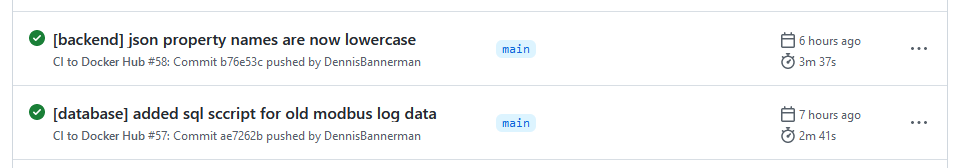
\includegraphics[scale=0.5]{github_actions_all_workflows} 
		\caption{Github Actions}
		\label{fig:github_actions_all_workflows}
	\end{figure}
	
	\subsubsection{Docker und Docker-Compose}
	\gls{docker} ist alleine schon vielfältig aber mit \gls{dockercompose} war das Deployen von jedem neuen Release ein Kinderspiel. Da wir die Datenbank, \gls{phpmyadmin} und unser \gls{springboot} Server auf drei \gls{container} verteilt haben konnte der \gls{springboot}t Server mit einem Befehl durch einen neuen Release ersetzt werden ohne dass wir die Daten verlieren und beim Fall unseres Hosts war das meist auch nur eine Dauer von maximal einer halben Minute bis der Server wieder erreichbar war.
	\begin{figure}[H]
		\centering
		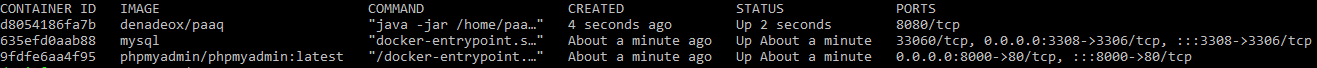
\includegraphics[scale=0.4]{docker} 
		\caption{Docker mit laufenden Containern}
		\label{fig:docker}
	\end{figure}
	
	\subsubsection{Swagger}
	Die mit \gls{openapi} zu bedienende Swagger Software schreckte uns Anfangs ein wenig zurück. Doch schnell erkannten wir das Potential und die Vielfältigkeit der Software die uns behilflich sein könnte. Mit Online Tools und ebenfalls eine SwaggerHub wird die Arbeit mit Swagger sehr unterstützt. Im Online Tool gibt es eine schöne Vorschau und der \gls{yaml} Code der geschrieben wird, wird auch in Echtzeit überprüft und man wird auch auf Fehler hingewiesen. Mit dem verbundenem SwaggerHub kann man sich auch von der \gls{api} von anderen inspirieren lassen.
		\begin{figure}[H]
		\centering
		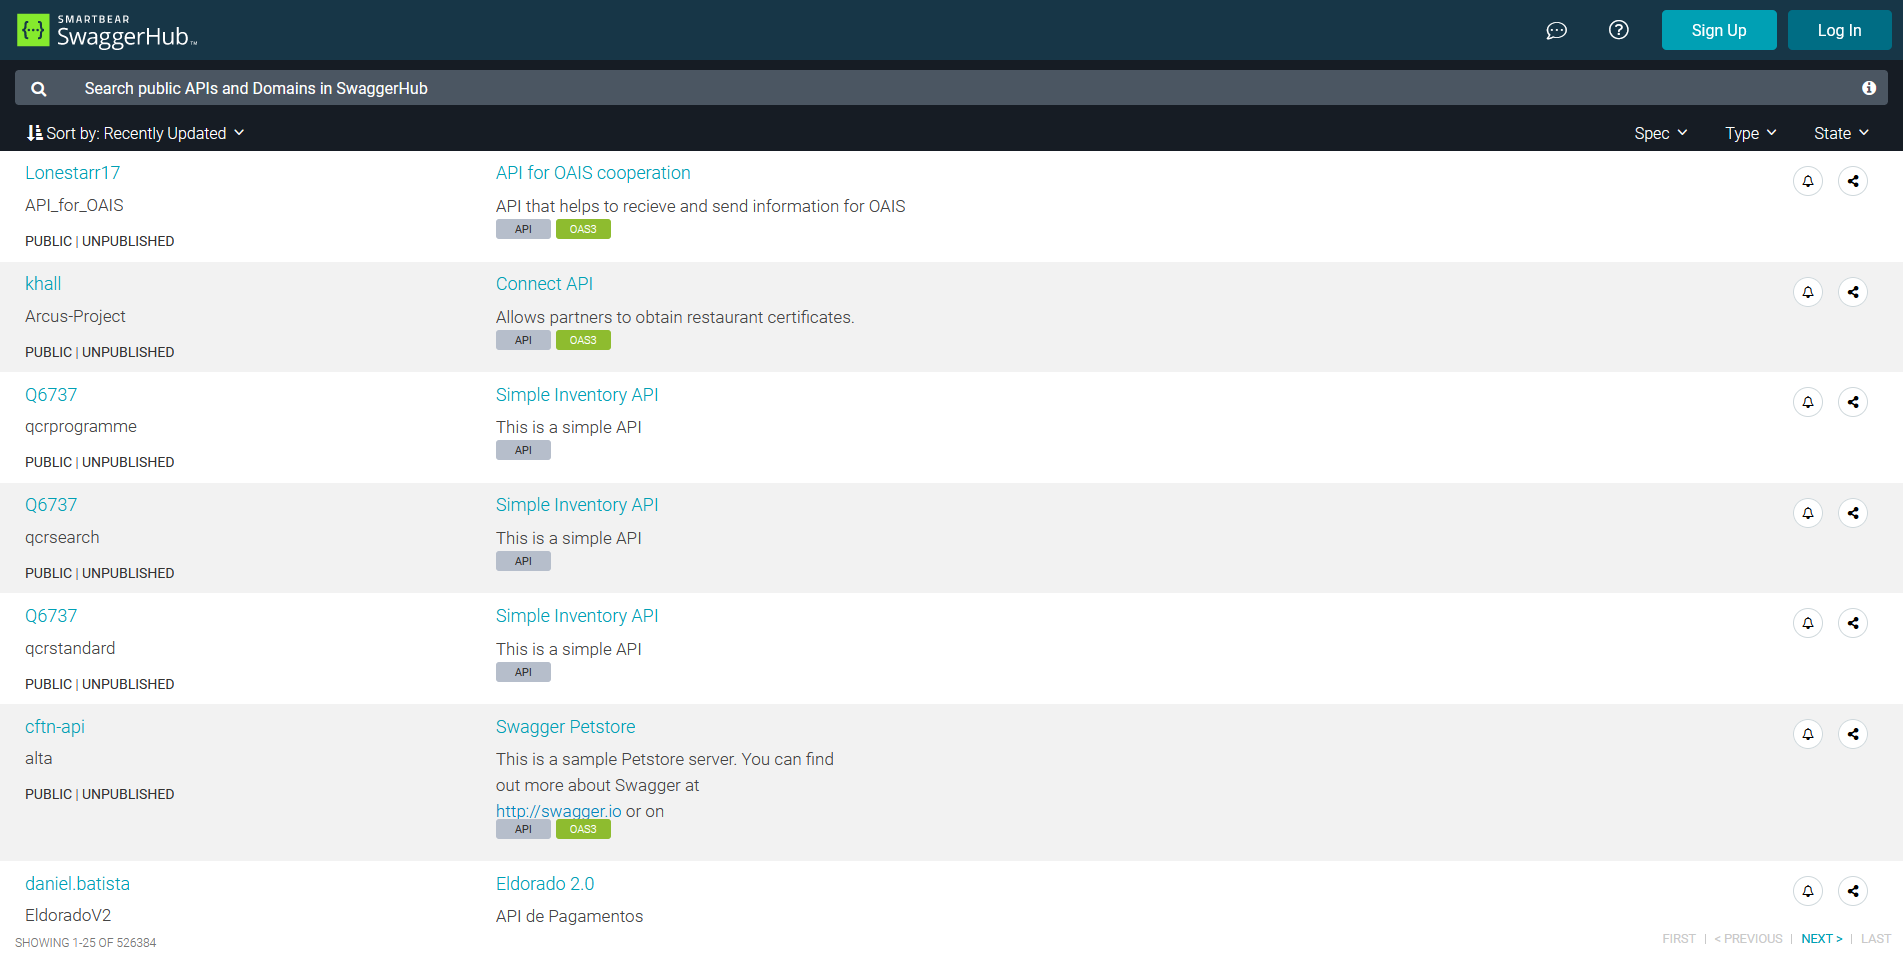
\includegraphics[scale=0.25]{swaggerhub} 
		\caption{SwaggerHub}
		\label{fig:swaggerhub}
	\end{figure}
	
	\subsubsection{Spring Boot}
	
	\subsubsection{Angular}
	
	\subsubsection{Sloppy Zone}
	
	\subsection{Bachelorarbeit Möglichkeiten}
	Weiterführende Möglichkeiten des Projektes bestehen. Unter anderem stehen Optionen offen, wie alle Logdateien als CSV zu exportieren um diese weiterzuverarbeiten.
	\\ \\
	Grössere weiterführende Projekte sind unter anderem ein Erkennungssystem für die Fische und die gesamte Umwelt im Tank. \\
	Folgende Punkte können zukünftig implementiert werden:
	\begin{itemize}
		\item Anzahl und Gewicht der Fische erkennen.
		\item Durch das Gewicht und die Anzahl die Fütterungsrate festlegen.
		\item Sauerstoffgehalt des Wassers erkennen und angezeigt werden. Damit man im Notfall jederzeit eingreifen kann.
		\item Gesundheit der Fische überwachen unter anderem:
		\begin{itemize}
			\item Körper und Flossenkonditionen des Fisches durch Kameras überwachen
			\item Schuppenprobleme, Deformierungen, Kiemenverfärbungen erkennen und frühzeitig warnen
		\end{itemize}
	\end{itemize}	
	Diese Punkte würden Bildbearbeitungsmethoden benötigen, welche diese Punkte erkennen können. Damit Massnahmen in den verschiedenen Fällen getroffen werden können. 
	\par 
	\begin{figure}[H]
		\centering
		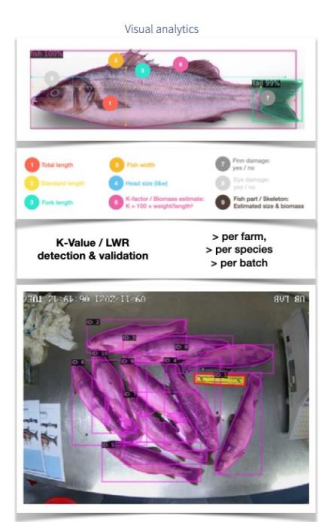
\includegraphics{../images/Imageprocessing} 
		\caption{Bildbearbeitungsmethoden}
		\label{fig:Imageprocessing}
	\end{figure}
	
	\par \noindent
	Hiermit werden weitere Möglichkeiten für Überwachungen eröffnet wie z.B:
	
	\begin{itemize}
		\item Verhalten 
		\item Sterblichkeit
		\item Platzgebrauch
		\item Gruppierungen
		\item Isolationen
		\item Schwimmgeschwindigkeit
		\item Körpergleichgewicht
	\end{itemize}
	\noindent
	Das würde bereits Videobearbeitung erfordern, um das Verhalten auf gewisse Aktionen zu erkennen. 
	
\end{document}